%Copyright 2014 Jean-Philippe Eisenbarth
%This program is free software: you can 
%redistribute it and/or modify it under the terms of the GNU General Public 
%License as published by the Free Software Foundation, either version 3 of the 
%License, or (at your option) any later version.
%This program is distributed in the hope that it will be useful,but WITHOUT ANY 
%WARRANTY; without even the implied warranty of MERCHANTABILITY or FITNESS FOR A 
%PARTICULAR PURPOSE. See the GNU General Public License for more details.
%You should have received a copy of the GNU General Public License along with 
%this program.  If not, see <http://www.gnu.org/licenses/>.

%Based on the code of Yiannis Lazarides
%http://tex.stackexchange.com/questions/42602/software-requirements-specification-with-latex
%http://tex.stackexchange.com/users/963/yiannis-lazarides
%Also based on the template of Karl E. Wiegers
%http://www.se.rit.edu/~emad/teaching/slides/srs_template_sep14.pdf
%http://karlwiegers.com
\documentclass{scrreprt}
\usepackage{listings}
\usepackage{graphicx}
\usepackage{underscore}
\usepackage[bookmarks=true]{hyperref}
\usepackage[utf8]{inputenc}
\usepackage[english]{babel}
\hypersetup{
    bookmarks=false,    % show bookmarks bar?
    pdftitle={Software Requirement Specification},    % title
    pdfauthor={Jean-Philippe Eisenbarth},                     % author
    pdfsubject={TeX and LaTeX},                        % subject of the document
    pdfkeywords={TeX, LaTeX, graphics, images}, % list of keywords
    colorlinks=true,       % false: boxed links; true: colored links
    linkcolor=blue,       % color of internal links
    citecolor=black,       % color of links to bibliography
    filecolor=black,        % color of file links
    urlcolor=blue,        % color of external links
    linktoc=page            % only page is linked
}%
\def\myversion{1.0 }
\date{}
%\title
\usepackage{hyperref}
\begin{document}

\begin{flushright}
    \rule{16cm}{5pt}\vskip1cm
    \begin{bfseries}
        \Huge{SOFTWARE REQUIREMENTS\\ SPECIFICATION}\\
        \vspace{1.9cm}
        for\\
        \vspace{1.9cm}
        Book Shop Automation Software\\
        \vspace{1.9cm}
        \LARGE{Version \myversion approved}\\
        \vspace{1.8cm}
        Presented by\\
        \vspace{0.5cm}
        Rameshwar Bhaskaran \textbf{(14CS30027)} \\
        Aditya Bhagwat \textbf{(14CS30002)} \\
		Group 55 \\        
        \vspace{1.3cm}
        IIT Kharagpur\\    
       
        \today\\
    \end{bfseries}
\end{flushright}

\tableofcontents

%\chapter*{Revision History}

%\begin{center}
 %   \begin{tabular}{|c|c|c|c|}
  %      \hline
	%    Name & Date & Reason For Changes & Version\\
     %   \hline
	  %  21 & 22 & 23 & 24\\
       % \hline
	   % 31 & 32 & 33 & 34\\
       % \hline
    %\end{tabular}
%\end{center}

\chapter{Introduction}

\section{Purpose}
The purpose of this document is to give a detailed description of the requirements for the “Book Shop Automation Software” (BAS) software. It will illustrate the purpose and complete declaration for the
 development of system. It will also explain system constraints, interface and interactions with other external applications. Unless
 otherwise stated, all requirements specified here are high priority and committed for release
 1.0.

\section{Document Conventions}
The document convention is very simple. All major section headings are in bold . Hyperlinks are indicated by blue bounding boxes.

\section{Intended Audience and Reading Suggestions}
This document is meant for the customers and the employees of the Book Shop. The document describes the workflow of the software and hence is extremely essential for all users to be well-acquainted with this document

\section{Project Scope}
In today's world, there arises a need to get things done quickly and efficiently. Customers find it difficult at times to find a book from book shops close to them . At the same time, the book shop owner wouldn't want to take a risk of losses due to stagnant stock. This issue is resolved by a neat mutually beneficial way by the software. It strives to be a fully independent entity with all necessary features to handle transactions and queries in a book shop. 
Also a need to automate tasks which need to be performed daily arises. In this case, the software reduces the risk and need of a third party to manually perform these mundane tasks.

\section{References}

\begin{itemize}
\item IEEE standard \href{http://www.cse.msu.edu/~cse870/IEEEXplore-SRS-template.pdf}{template} for IEEE standard 

\item Fundamentals of Software Engineering by R.Mall
\end{itemize}

\section{Definitions, Acronyms and Abbreviations Used}
\begin{itemize}
\item \textbf{BAS}   Book Shop Automation Software
\item \textbf{SRS}   Software Requirements Specifications
\item \textbf{ISBN}   International Standard Book Number is a unique 13 digit code for each book. Contains  information related to Title, Publisher and Group etc. Different Editions will have different ISBN and  ISBN for different copies of same book will be same.

\end{itemize}
\chapter{Overall Description}

\section{Product Perspective}
The BAS is an independently functioning system that automates manual  tasks in a Book Shop like answering customer queries, billing, making sales statistics, planning for further orders etc. The system handles and stores all necessary records of books in a database. The user interface is simple for any user to understand when he/she uses it for the first time itself . The software also analyses data and presents it in a useful form for any important stakeholder like the owner and his business associates to take important decisions.
\section{Product Functions}
The BAS performs these major tasks:
\\
\begin{itemize}
\item \textbf{Query for books:}\\
The customer can query for availability of the book by entering its title or the author's name. On availability , the BAS shows the rack number and the number of copies in stock.

\item \textbf{Request for book:}\\
If the query for the book fails, then the customer has an option of requesting for the book shop to order the book in question by entering the full details of the book (Name, Author's name, ISBN code,Publisher's name ). Depending on the number of requests, the Manager may decide to order the book.

\item \textbf{Update stock and inventory:}\\
When the customer confirms the book, the BAS updates the inventory. Also in case of new arrivals/defective pieces, the BAS updates accordingly.

\item \textbf{View requests:}\\
The Manager can view the number of requests for the books and decide on the course of action to be taken.

\item \textbf{Generate sales receipt:}\\
	To complete the transaction, the BAS generates a sales receipt for endorsing the 	transaction.

\item \textbf{Generate sales statistics:}\\	
	The BAS generates sales statistics based on transactions between any given period. This 	feature is used by the owner and any other authorised person. This also helps in finding 	the inventory level.                                      

\item \textbf{Print the list of books to be bought depending on the inventory level:}\\	
	Every day the book shop owner would give a command for the BAS to print
 the books 	which have fallen below the threshold and the number of copies to be procured 	along 	with the full
 address of the stockist.
 
 \end{itemize}
\section{User Classes and Characteristics}
 Main class has the access to information as it contains aggregations of many class objects and is the most privileged in the sense of access. Cart is used very frequently in conjunction with SalesClerk to buy books and print receipts. This is the most general function of the software.

The user classes in this project are : \\ 
\begin{itemize}

\item  \textbf{Book :}\\ This class is central to this project. It stores those fields that characterize a Book object such as it's name, author's name, price, publisher, which rack it is kept on and so on. This implies that there can only be one book object per name - there will be one instance of the Book object “The Alchemist” irrespective of the number of copies of that book available. It's member functions give access to it's fields and allow us to change some mutable fields like number of copies available. This is the biggest class and holds the most amount of information.

\item  \textbf{Employee :} \\This class is derived multiple times to create sub-classes like sales clerk, manager and owner . These sub-classes allow us to implement the organizational hierarchy of the book shop.

\item    \textbf{SalesDay :} \\This class allows us to maintain an account of all the sales that take place during working day.

\item \textbf{NotInCollection :}\\  NotInCollection is the order request that contains the details of the book as specified by the customer.

\item \textbf{Cart :}\\ A customer may choose more than one book to buy in one transaction (and more than one copy per book). The cart maintains the list of books he/she wishes to buy.

\item \textbf {Main:}\\ This is the main application class that binds everything together. It contains the arrays of Book objects and registered employees. It also contains information regarding the books that have fallen below the threshold stock level and the books that are in demand but not a part of the collection. The sales statistics are also maintained in this class.

\item \textbf{SalesDay:}\\This is a very important class that stores the sales statistics for the day. Useful to get an overall picture of the sales statistics of a period and derive useful information from it.
\item \textbf{Other auxiliary classes :} \\Publisher and vendor classes have been introduced to better implement the Book class. Each vendor may house books of multiple publishers. Many books may have the same publisher.

\end{itemize}

\section{Operating Environment}
This software is built in Java and will run on Linux ,Windows and any other platforms which have a JVM pre-installed.As for hardware, it may require a printer to print out the sales receipt generated.

\section{Design and Implementation Constraints}
As the BAS needs to handle large number of books, that may lead to lagging of the system to handle data from database. 
A linear time algorithm may itself lose efficiency in such cases. Logarithmic time algorithms can be used ,but they will compromise on the memory used.

\section{User Documentation}
As the product is presently in prototype stage, the documentation is not available. Once the full software is built, the user documentation may be presented In html or pdf formats.

\section{Assumptions and Dependencies}

We have assumed that the computer used in the book shop is perfectly working and has a perfectly working Java runtime environment and JVM installed. As the software is built using Java, it is safely assumed that appropriate software is installed.\\
Coming to the problem statement, in order to give a more general perception to the problem in hand, there are other types of employees other than the Manager and Sales Clerk. 

\chapter{External Interface Requirements}
\section{User Interfaces}
The Book Shop Automation software is implemented on a single application window. There are multiple simultaneous users of the software so the interface necessarily has to cater to both the customer and the employee logged in currently. On the (default) main screen the logged in employee's name and job profile is displayed at the top right. There are 2 buttons for login and logout. Clicking the login button results in a login window popping up. Logging in makes us return to the main screen. The main screen will, most importantly, consist of a search bar on the top with a label that asks the user to enter either the author's name or the book title. There is space for displaying relevant search results below this search bar. Depending upon the employee logged in there will be buttons on the bottom to the left (outside the search result space) pertaining to his/her responsibilities. Clicking these buttons may pop windows (or change the panel in the same window) to perform required activities.\\


After the user enters the search query and results are displayed he has the option to view the book which redirects him to a window where he can view it's details. Here he can choose the number of copies he wishes to buy, and he returns back to the search page. The books chosen are added to the 'My Cart' sub-panel on the right of the main screen. There will be a button to finalize cart and proceed to payment which will change the screen. At this point the sales clerk will take over. Here, he will enter the ISBN code of each book and finally press the button to complete the transaction and print out the bill and return to the main screen again.\\

If the queried book has run out of stock or has insufficient stock to complete the transaction, the customer  can create a new book request or increment a pre-created request. If the search result is empty, then the customer is given the option to enter the relevant details of the desired book and create a new-book-request. The manager can view  both these requests by clicking a button visible to him on the main screen, which redirects to a new screen. The owner can view sales statistics similarly.

\section{Hardware Interfaces}
As indicated before ,the only external hardware the software needs is a printer. This can be accessed using the Java 2D printing API or any other suitable API. 

\section{Software Interfaces}

This software is a standalone application with the its own user interface handling user interaction fully. When necessary data needs to be retrieved/added/modified, then a connection is made to the database via a driver. All tools and libraries used in the software are open-source. 

\section{Communications Interfaces}

The software doesn't require internet to function for its requirements. However it may require internet to implement certain features like a global signin/signup option wherein the users may be spread over. In such cases, the internet connection must be present and must allow TCP (Transfer Control Protocol) and HTTP.


\chapter{System Features}
The BAS is a multi-faceted software that supports multiple features. The following are some of the important features that are implemented. \\


\section{Query for book}
The main objective/highlight of the software is to enable query for the books.
\subsection{Description and Priority}
High priority feature. The search used is linear ,hence the software may lag behind for large number of books. 

\subsection{Stimulus/Response Sequences}
The user(customer) will enter the name of the author/title of the book to get the list of matching books. 

\subsection{Functional Requirements}
The feature requires a database connection and provision to get user input .The user needs to enter the appropriate keywords to get the book. To help with suggestions, the minimum edit distance algorithm and various string matching algorithms are deployed. 



\section{Display details}

This feature helps display the details of the book like title,rack number and the number of copies left. 
\subsection{Description and Priority}
High priority feature. This will decide whether the user needs to buy the book and carry out the transaction. 

\subsection{Stimulus/Response Sequences}
This feature is used only when the user presses the query button as well as the database has a matching entry with the user input.

\subsection{Functional Requirements}
The feature requires a database connection and an appropriate  UI wherein the details can be displayed.

\begin{figure}
  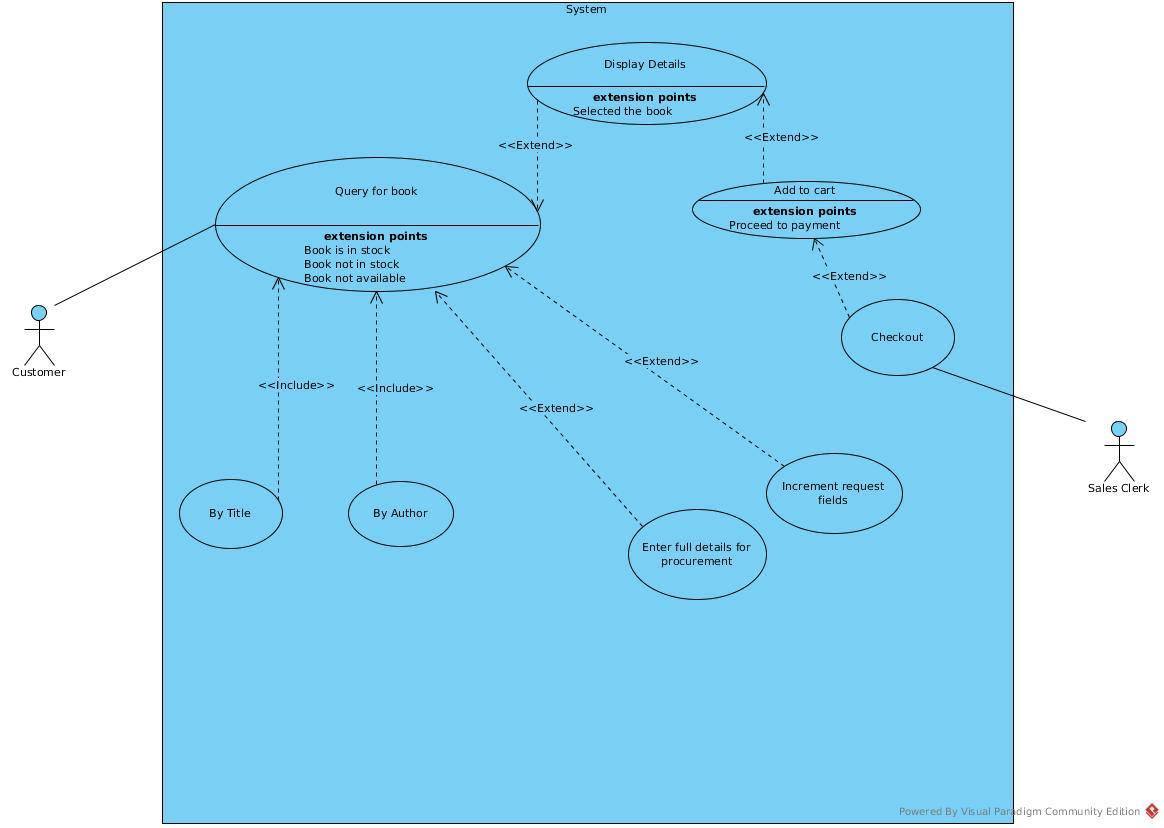
\includegraphics[width=\linewidth]{Customer.jpg}
  \caption{Use case diagram of the software.}
  \label{fig:usecase}
\end{figure}

\section{Increment request field}

This feature helps requesting the manager to order more copies of the book that is presently not in stock. 
\subsection{Description and Priority}
High priority feature. This would not only help the shop improve its business, but also would help prevention of stagnant stock. 

\subsection{Stimulus/Response Sequences}
This feature is used only when the user presses the query button and the database has the book record but number of its copies is 0. Then the UI further shows a dialog box wherein the user is offered to increment request field.

\subsection{Functional Requirements}
The feature requires a database connection and an appropriate  UI wherein the details can be displayed.

\begin{figure}
  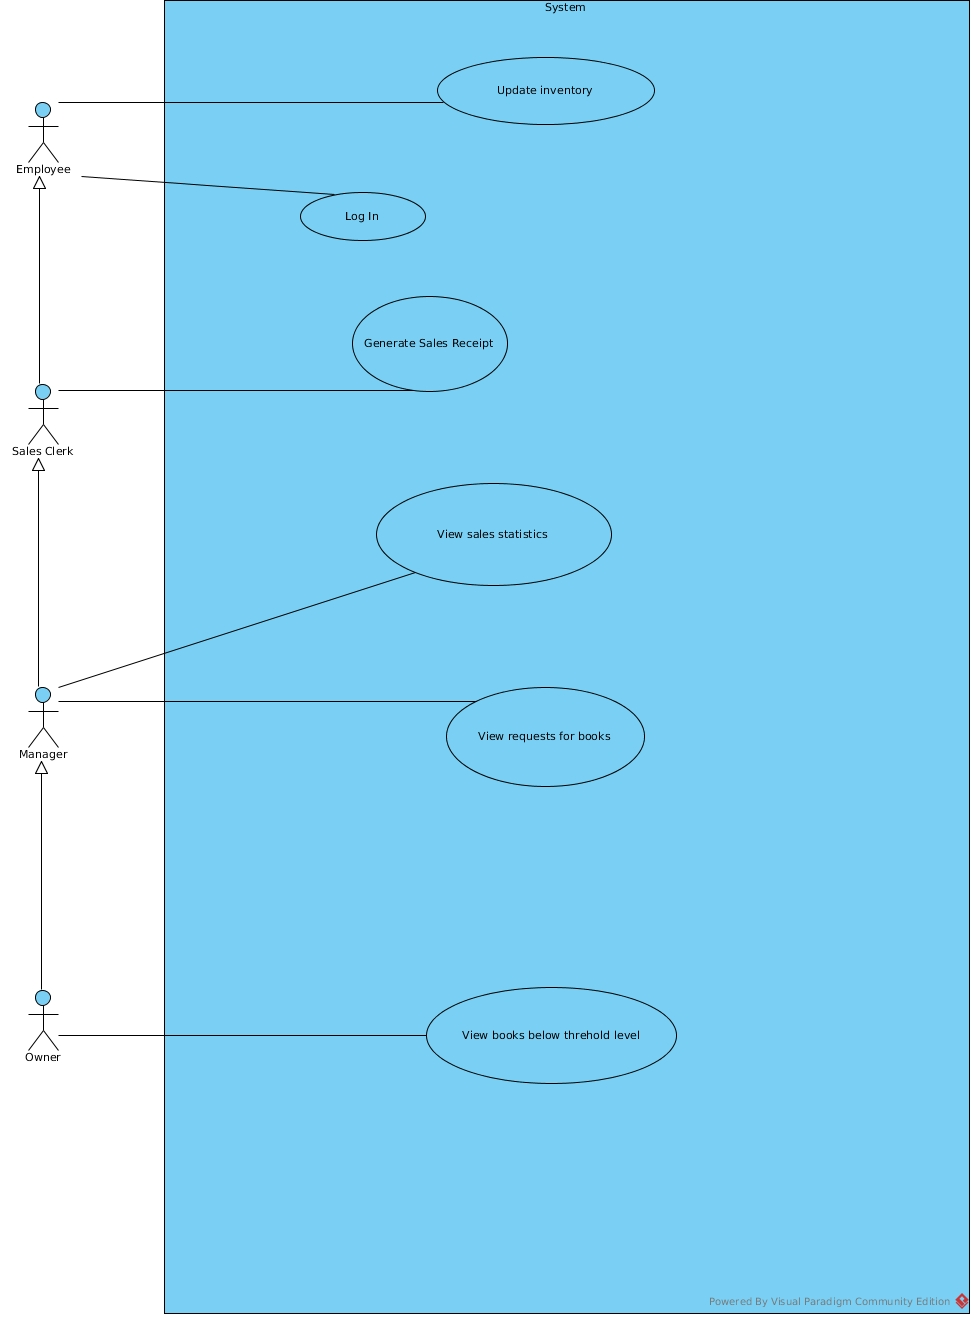
\includegraphics[width=\linewidth]{General Employee.jpg}
  \caption{Use case diagram of the software.}
  \label{fig:usecase}
\end{figure}

\section{Request for new book}

This feature helps requesting the manager to order more copies of the book that hasn't been sold yet. 
\subsection{Description and Priority}
High priority feature. This feature is important for improving the shop's inventory.

\subsection{Stimulus/Response Sequences}
This feature is used only when the user presses the query button and the database doesn't have such a book record. In such a case, the software takes in customer input for details of the book like the ISBN code and name. This is forwarded.

\subsection{Functional Requirements}
The feature requires a database connection and an appropriate  UI wherein provision for user input is present.

\section{Update inventory}

This feature helps employees to update stock details once stock arrives/transactions are made. 
\subsection{Description and Priority}
High priority feature. This feature is integral for getting the inventory updated. This feature is crucial for every other major feature to work right.

\subsection{Stimulus/Response Sequences}
This feature is used only when new stock has arrived. Also it is used in cases where books are sold or is defective.

\subsection{Functional Requirements}
This feature requires a database connection and only employees of the shop are allowed to change the inventory.

\section{Add to cart}

This feature helps customers to add books to their cart to get the transactions done together.
\subsection{Description and Priority}
Medium priority feature. This feature is a important add-on to improve user experience. However its absence won't affect the basic functioning of the software.

\subsection{Stimulus/Response Sequences}
This feature is used only when new stock has arrived. Also it is used in cases where books are sold or is defective.

\subsection{Functional Requirements}
This feature requires a database connection and only employees of the shop are allowed to change the inventory.


\section{View statistics}

This feature helps the owner and manager to view sales statistics to make important decisions.
\subsection{Description and Priority}
High priority feature. It is used to make the sales data in a more comprehendable and better fashioned way.

\subsection{Stimulus/Response Sequences}
This feature is invoked when the manager/owner clicks the "View Statistics" button. 

\subsection{Functional Requirements}
This feature requires a database connection and only the managers and the owner are allowed to use this feature. Also this feature may require external graphing libraries or plot visualising tools.

\section{View requests}

This feature helps the manager to review both incremental requests and well as requests for new books.
\subsection{Description and Priority}
High priority feature. It helps in analysing the stock needed for procurement.

\subsection{Stimulus/Response Sequences}
This feature is invoked when the manager/owner clicks the "View incremental requests" button and "View new book requests" button. 

\subsection{Functional Requirements}
This feature requires a database connection and only the managers and higher authorities are allowed to use this feature. 


\chapter{Other Nonfunctional Requirements}

\section{Performance Requirements}

The software is supposed to be designed for a small to medium sized book shop. The book shop is assumed to house a few thousand books (or less) at any given point in time. Hence search results are supposed to be almost instantaneous. This goes for all the operations that a customer may perform, including updating the cart and requesting for a new book. The same can be said about printing sales receipt and viewing order requests. Displaying the sales statistics is the only computationally heavy operation and may potentially take a few minutes but only if the period entered is too large, say 10 years.

\section{Safety Requirements}
All exceptions have to be properly handled so that the application doesn't crash under any circumstances and no data is lost. Because the software requirements necessitate the operation of a cron job, that operates on data generated during a day, crashes can potentially lead to a great losses of information to the owner. Safeguards must be put in place so that this never happens.

\section{Security Requirements}
The BAS handles very sensitive data including personal details of employees and customers and details of transactions. Such data needs to be suitably 'abstracted' to prevent misuse. No external software should be given access to the internal parts/modules of the software, as that may lead to its misuse. 

\section{Software Quality Attributes}
The software must include user authentication for all types of operation besides operation by the customer. Different classes of employees have different accessibility privileges and this must be strictly upheld for the data to remain safe.

\section{Business Rules}
The software must have wide adaptability and reusability. Many book shops choose to also sell music CDs, DVDs and cassettes. Some choose to also keep magazines and journals depending on their customer base. The software must be modularized enough to allow for this. Since it will be operated on by non-professionals (both the lay employee as well as customers) ease of use is vital. It must be robust and maintainable as it is possible that it may be used continuously for many years.


%\chapter{Other Requirements}

\end{document}

